\documentclass{article}
\usepackage{amsmath}
\usepackage{amsthm}
\usepackage{amssymb}
\usepackage{graphicx}
\usepackage{color}
%\include{macros}
%\usepackage{floatflt}
%\usepackage{graphics}
%\usepackage{epsfig}
\usepackage[colorlinks,linkcolor=red,anchorcolor=blue,citecolor=green]{hyperref}
\usepackage{epstopdf}

\usepackage[UTF8]{ctex}
\usepackage{verbatim}
\usepackage[backend=bibtex,style=authoryear,natbib=true,backref=true]{biblatex}

\theoremstyle{definition}
\newtheorem{theorem}{定理}[section]
\newtheorem{lemma}[theorem]{引理}
\newtheorem{proposition}[theorem]{Proposition}
\newtheorem{corollary}[theorem]{Corollary}

\theoremstyle{definition}
\newtheorem*{definition}{Definition}
\newtheorem*{example}{Example}

\theoremstyle{remark}
\newtheorem*{remark}{Remark}
\newtheorem*{note}{Note}
\newtheorem*{exercise}{Exercise}

\setlength{\oddsidemargin}{-0.25 in}
\setlength{\evensidemargin}{-0.25 in} \setlength{\topmargin}{-0.25
in} \setlength{\textwidth}{7 in} \setlength{\textheight}{8.5 in}
\setlength{\headsep}{0.25 in} \setlength{\parindent}{0 in}
\setlength{\parskip}{0.1 in}

\newcommand{\homework}[4]{
\pagestyle{myheadings} \thispagestyle{plain}
\newpage
\setcounter{page}{1} \noindent
\begin{center}
\framebox{ \vbox{\vspace{2mm} \hbox to 6.28in { {\bf
THU-70250403,~Convex~Optimization~(Fall 2018) \hfill Homework: #4}}
\vspace{6mm} \hbox to 6.28in { {\Large \hfill #1 \hfill} }
\vspace{6mm} \hbox to 6.28in { {\it Lecturer: #2 \hfill} }
\vspace{2mm} \hbox to 6.28in { {\it Student: #3 \hfill} }
\vspace{2mm} } }
\end{center}
\markboth{#1}{#1} \vspace*{4mm} }

\addbibresource{./ref/ref.bib} % The filename of the bibliography

\begin{document}

\homework{L1-TWSVM}{Shuning Wang, Li Li \hspace{5mm} {\tt swang@tsinghua.edu.cn \tt
li-li@tsinghua.edu.cn }}{闫茹钰, 喻望, 张芙作, 郑洁, 朱榕平 \hspace{5mm} {\tt }}{2}

% zhangfz15@mails.tsinghua.edu.cn

\section{TWSVM}

TWSVM (孪生支持向量机) 是 Jayadeva 等人于2007年提出的一种改进的双分界面支持向量机,用于解决二分类问题。与传统的支持向量机 (SVM) 不同,TWSVM 为每一类的数据点单独建立一个分类面,其优化策略为,使同一类的数据点尽可能集中的围绕在该类分类面的周围,并且远离另一类数据的分类面。所以 TWSVM 需要解决两个二次规划问题,得到两个不平行的分类面,但是同一类的数据要作为另一个二次规划问题的约束条件,反之亦然。

TWSVM 需要求解以下两个二次优化问题:
\begin{align}
\begin{split}
\label{ts1}
\min_{\mathbf{w}_1,b_1} \; & \frac{1}{2}\|\mathbf{Aw}_1+\mathbf{e}_1b_1\|_2^2+c_1\mathbf{e}_2^T\mathbf{q}_1 \\
s.t.\; & -(\mathbf{Bw}_1+\mathbf{e}_2b_1)+\mathbf{q}_1 \geq \mathbf{e}_2,\mathbf{q}_1\geq 0
\end{split}
\\
\begin{split}
\label{ts2}
\min_{\mathbf{w}_2,b_2} \; & \frac{1}{2}\|\mathbf{Bw}_2+\mathbf{e}_2b_2\|_2^2+c_2\mathbf{e}_1^T\mathbf{q}_2 \\
s.t. \; & (\mathbf{Aw}_2+\mathbf{e}_1b_2)+\mathbf{q}_2\geq \mathbf{e}_1, \mathbf{q}_2\geq 0
\end{split}
\end{align}
其中,$\mathbf{A}_{m_1 \times n}=(\mathbf{a}_1^{(1)},\mathbf{a}_2^{(1)},\ldots,\mathbf{a}_{m_1}^{(1)})^T$ 表示 $m_1$ 个正样本,$\mathbf{B}_{m_2 \times n }=(\mathbf{b}_1^{(2)},\mathbf{a}_2^{(2)},\ldots,\mathbf{a}_{m_2}^{(2)})^T$ 表示 $m_2$ 个负样本,$\mathbf{e}_1$ 和 $\mathbf{e}_2$ 表示相应维数的单位变量,$||\cdot||_2$ 表示L2范数,$\mathbf{q}_1, \, \mathbf{q}_2$ 是松弛向量,$c_1, \, c_2$ 是非负惩罚系数,分别为正样本和负样本的平衡因子,可以用来解决正负样本个数不同的问题。通过求解以上两个优化问题,可以分别得到两个不平行的超平面:
\begin{equation}
\mathbf{x}^T\mathbf{w}_1+b_1=0, \quad \mathbf{x}^T\mathbf{w}_2+b_2=0
\end{equation}
当有一个新的点 $\mathbf{x}$,计算其到两个超平面的垂直距离,如果它距离超平面 $\mathbf{x}^T\mathbf{w}_1+b_1=0$ 的距离小于它到超平面 $\mathbf{x}^T\mathbf{w}_2+b_2=0$ 的距离,则将该点归入正类,否则它属于负类。

我们也可以得到问题 (\ref{ts1})、(\ref{ts2}) 的 Wolfe 对偶问题:
\begin{align}
\begin{split}
\max\limits_{\pmb{\alpha}} \; & \mathbf{e}_2^T \pmb{\alpha}-\frac{1}{2}\pmb{\alpha}^T\mathbf{G}(\mathbf{H}^T\mathbf{H})^{-1}\mathbf{G}^T\pmb{\alpha} \\
s.t. \; & 0 \leq \pmb{\alpha}\leq c_1 \mathbf{e}_2
\end{split}
\\
\begin{split}
\max\limits_{\pmb{\beta}} \; & \mathbf{e}_1^T \pmb{\beta}-\frac{1}{2}\pmb{\beta}^T\mathbf{H}(\mathbf{G}^T\mathbf{G})^{-1}\mathbf{H}^T\pmb{\beta} \\
s.t. \; & 0 \leq \pmb{\beta} \leq c_2\mathbf{e}_1
\end{split}
\end{align}
其中 $\mathbf{\alpha} \in R^{m_2}$ 和 $\mathbf{\beta}\in R^{m_1}$ 是拉格朗日乘子,可以利用 $\mathbf{\alpha}$ 和 $\mathbf{\beta}$ 得到两个不平行的超平面:
\begin{align}
\begin{split}
\mathbf{z}_1 &= (\mathbf{w}^T_1b_1)^T = -(\mathbf{H}^T\mathbf{H})^{-1} \mathbf{G}^
T\pmb{\alpha} \\
\mathbf{z}_2 &= (\mathbf{w}^T_2b_2)^T = (\mathbf{G}^T\mathbf{G})^{-1} \mathbf{H}^T\pmb{\beta}
\end{split}
\end{align}
由于逆矩阵 $(\mathbf{H}^T\mathbf{H})^{-1}$ 和 $(\mathbf{G}^T\mathbf{G})^{-1}$ 可能带来奇异问题,为防止矩阵奇异,可以加入一个正则项 $\varepsilon \mathbf{I}$,$\varepsilon$ 是一个足够小的正数。这样可以保证 $(\mathbf{H}^T\mathbf{H}+\varepsilon \mathbf{I})^{-1}$ 和 $(\mathbf{G}^T\mathbf{G}+\varepsilon \mathbf{I})^{-1}$ 正定,从而不会出现奇异问题。

图 \ref{twsvm1} 是对TWSVM的几何解释。
\begin{figure}[ht]
\centering
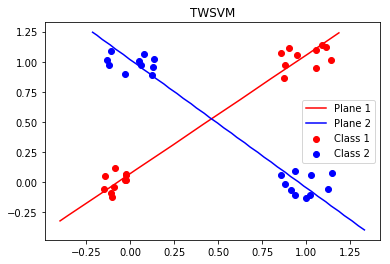
\includegraphics[height=5cm]{./img/TWSVM-img.png}
\caption{TWSVM}
\label{twsvm1}
\end{figure}

\section{收敛性证明}
\begin{lemma}
   对任意非零向量 $\mathbf{u},\mathbf{u}^p\in\mathbb{R}^1$,有以下不等式:
   \begin{equation}
   \|\mathbf{u}\|_{1}-\frac{\|\mathbf{u}\|^{2}_{1}}{2\|\mathbf{u}^p\|_{1}}\le
   \|\mathbf{u}^p\|_{1}-\frac{\|\mathbf{u}^p\|^{2}_{1}}{2\|\mathbf{u}^p\|_{1}}
   \label{yw1}
   \end{equation}
\end{lemma}

证明:
\begin{equation}
\begin{aligned}
&(\sqrt{\mathbf{v}}-\sqrt{\mathbf{v^p}})^2\ge0
\Rightarrow\mathbf{v}-2\sqrt{\mathbf{vv}^p}+\mathbf{v}^p\ge0\\
&\Rightarrow\sqrt{\mathbf{v}}-\frac{\mathbf{v}}{2\sqrt{\mathbf{v}^p}}\le
\frac{\sqrt{\mathbf{v}^p}}{2}
\Rightarrow\sqrt{\mathbf{v}}-\frac{\mathbf{v}}{2\sqrt{\mathbf{v}^p}}\le
\sqrt{\mathbf{v}^p}-\frac{\mathbf{v}^p}{2\sqrt{\mathbf{v}^p}}
\end{aligned}
\label{yw2}
\end{equation}
将式 \eqref{yw2} 中的 $\mathbf{v}$ 和 $\mathbf{v}^p$ 替换为 $\|\mathbf{u}\|^{2}_{1}$ 和 $\|\mathbf{u}^p\|^{2}_{1}$,即得到式 \eqref{yw1}。

\begin{theorem}
   算法1在每步迭代中都使问题 的目标值单调递减。
\end{theorem}

证明:首先,用以下等式重写\ 中的问题:
\begin{equation}
\mathbf{z}^{(p+1)}_{1}=\mathop{\arg\min}_{\mathbf{z}_{1}}
\frac{1}{2}\mathbf{z}^{T}_{1}\mathbf{H}^{T}\mathbf{D}^{T}_{1}\mathbf{H}\mathbf{z}_{1}+
c_{1}\mathbf{e}^{T}_{2}\mathop{\max}(0,\mathbf{e}_{2}+\mathbf{Gz}_{1})
\label{yw3}
\end{equation}
即:
\begin{equation}
\mathbf{z}^{(p+1)}_{1}=\mathop{\arg\min}_{\mathbf{z}_{1}}
\frac{1}{2}(\mathbf{Hz}_{1})^{T}\mathbf{D}^{p}_{1}\mathbf{Hz}_{1}+
c_{1}\mathbf{e}^{T}_{2}\mathop{\max}(0,\mathbf{e}_{2}+\mathbf{Gz}_{1})
\label{yw4}
\end{equation}
因此,在第 $(p+1)$ 步迭代中,有
\begin{equation}
\begin{aligned}
&\frac{1}{2}(\mathbf{Hz}^{(p+1)}_{1})^{T}\mathbf{D}^{p}_{1}(\mathbf{Hz}^{(p+1)}_{1})+
c_{1}\mathbf{e}^{T}_{2}\mathop{\max}(0,\mathbf{e}_{2}+\mathbf{Gz}^{(p+1)}_{1})\\
&\le\frac{1}{2}(\mathbf{Hz}^{p}_{1})^{T}\mathbf{D}^{p}_{1}(\mathbf{Hz}^{p}_{1})+
c_{1}\mathbf{e}^{T}_{2}\mathop{\max}(0,\mathbf{e}_{2}+\mathbf{Gz}^{p}_{1})
\end{aligned}
\label{yw5}
\end{equation}
将式 \eqref{yw1} 中的 $\mathbf{u}$ 和 $\mathbf{u}^p$ 替换为 $\mathbf{Hz}^{(p+1)}_{1}$ 和 $\mathbf{Hz}^{p}_{1}$,可以得到:
\begin{equation}
\|\mathbf{Hz}^{(p+1)}_{1}\|_{1}-\frac{\|\mathbf{Hz}^{(p+1)}_{1}\|^{2}_{1}}{2\|\mathbf{Hz}^{p}_{1}\|_{1}}\le
\|\mathbf{Hz}^{p}_{1}\|_{1}-\frac{\|\mathbf{Hz}^{p}_{1}\|^{2}_{1}}{2\|\mathbf{Hz}^{p}_{1}\|_{1}}
\label{yw6}
\end{equation}
因此可得如下不等式:
\begin{equation}
\sum^{m_1}_{i=1}(\left|\mathbf{h}^{T}_{i}\mathbf{z}^{(p+1)}_1\right|-
\frac{(\mathbf{h}^{T}_{i}\mathbf{z}^{(p+1)}_1)^2}
{2\left|\mathbf{h}^{T}_{i}\mathbf{z}^{p}_{1}\right|})\le
\sum^{m_1}_{i=1}(\left|\mathbf{h}^{T}_{i}\mathbf{z}^{p}_1\right|-
\frac{(\mathbf{h}^{T}_{i}\mathbf{z}^{p}_1)^2}
{2\left|\mathbf{h}^{T}_{i}\mathbf{z}^{p}_{1}\right|})
\label{yw7}
\end{equation}
该式可被简化为:
\begin{equation}
\begin{aligned}
&\|\mathbf{Hz}^{(p+1)}_{1}\|_{1}-\frac{1}{2}(\mathbf{Hz}^{(p+1)}_{1})^{T}\mathbf{D}^{p}_{1}(\mathbf{Hz}^{(p+1)}_{1})\\
&\le\|\mathbf{Hz}^{p}_{1}\|_{1}-\frac{1}{2}(\mathbf{Hz}^{p}_{1})^{T}\mathbf{D}^{p}_{1}(\mathbf{Hz}^{p}_{1})     \end{aligned}
\label{yw8}
\end{equation}
综合式 \eqref{yw5} 和 \eqref{yw8},可得:
\begin{equation}
\begin{aligned}
&\|\mathbf{Hz}^{(p+1)}_{1}\|_{1}+c_{1}\mathbf{e}^{T}_{2}\mathop{\max}(0,\mathbf{e}_{2}+\mathbf{Gz}^{(p+1)}_{1})\\
&\le\|\mathbf{Hz}^{p}_{1}\|_{1}+c_{1}\mathbf{e}^{T}_{2}\mathop{\max}(0,\mathbf{e}_{2}+\mathbf{Gz}^{p}_{1})
\end{aligned}
\label{yw9}
\end{equation}
因为\ 中的问题恒小于零,因此算法1收敛,\eqref{yw9} 中的不等式成立。这表示\ 中的目标值随迭代递减,直到算法收敛。
\begin{theorem}
算法1收敛至问题\ 的一个局部最优解。
\end{theorem}
证明:问题\ 的拉格朗日函数如下:
\begin{equation}
L_{2}(\mathbf{z}_{1},\mathbf{q}_{1})=\frac{1}{2}\|\mathbf{Hz}_{1}\|_{1}+
c_{1}\mathbf{e}^{T}_{2}\mathbf{q}_{1}-\mathbf{\alpha}^{T}(-\mathbf{Gz}_{1}+\mathbf{q}_{1}-\mathbf{e}_{2})
-\mathbf{\beta^{T}q}_{1}
\label{yw10}
\end{equation}
其中,$\mathbf{\alpha}$ 和 $\mathbf{\beta}$ 是拉格朗日乘子向量。通过对其求导并取零,可以得到问题\ 的 KKT 条件:
\begin{equation}
\mathbf{H}^{T}\mathbf{D}_{1}\mathbf{Hz}_{1}+\mathbf{G\alpha}=0,
c_{1}\mathbf{e}_{2}-\mathbf{\alpha}-\mathbf{\beta}=0
\label{yw11}
\end{equation}
在算法1的每步迭代中,寻找问题\ 中的最优 $\mathbf{z}^{(p+1)}_{1}$ 。因此,算法1的收敛解满足问题的 KKT 条件。接下来,定义算法1中问题\ 的拉格朗日函数如下:
\begin{equation}
L_{3}(\mathbf{z}_{1},\mathbf{q}_{1})=\frac{1}{2}\mathbf{H}^{T}\mathbf{D}_{1}\mathbf{Hz}_{1}+
c_{1}\mathbf{e}^{T}_{2}\mathbf{q}_{1}-\mathbf{\alpha}^{T}(-\mathbf{Gz}_{1}+\mathbf{q}_{1}-\mathbf{e}_{2})
-\mathbf{\beta^{T}q}_{1}
\label{yw12}
\end{equation}
同样对其求导并取零,得到:
\begin{equation}
\mathbf{H}^{T}\mathbf{D}_{1}\mathbf{Hz}_{1}+\mathbf{G\alpha}=0,
c_{1}\mathbf{e}_{2}-\mathbf{\alpha}-\mathbf{\beta}=0
\label{yw13}
\end{equation}
根据算法1中 $\mathbf{D}_{1}$ 的定义,等式 \eqref{yw11} 和 \eqref{yw13} 在算法1收敛时成立。这说明算法1的收敛解 $\mathbf{z}^{(p+1)}_{1}$ 满足问题\ 的KKT条件,是问题\ 的一个局部最优解。

\section{数值实验}

类似论文原文,我们使用\emph{异或问题}测试 L1-TWSVM 算法的正确性。由于异或问题比较简单,直接采用本地随机生成的数据集。本次实验分别以点 $(0,\,0),\, (0,\,1),\, (1,\,0),\, (1,\,1)$ 为中心,范围 $[\pm 0.15,\, \pm 0.15]$ 内均匀产生 10 个样本点;再手动添加两个离群点 $(1.2,\, -0.3),\, (-0.3,\, -0.3)$。得到数据散点图如图 \ref{data_points} 所示。

\begin{figure}[ht]
\centering
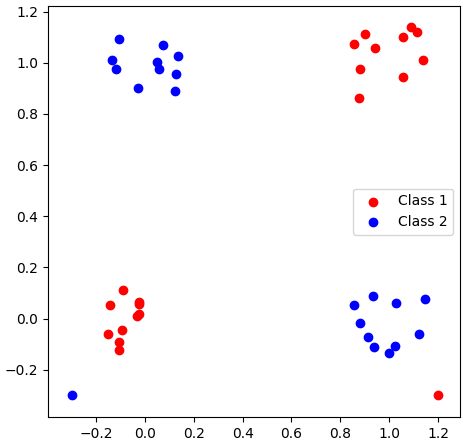
\includegraphics[width=0.35\textwidth]{./img/datas.png}
\caption{数据散点图}
\label{data_points}
\end{figure}

实验代码采用 \verb|Python| 编写,调用 \verb|cvxpy| \parencite{cvxpy} 求解凸优化问题,详细代码见附录 \ref{append_code}。首先不添加离群点,观察 TWSVM 与 L1-TWSVM 拟合超平面的效果对比,得到输出:
\begin{verbatim}
Init solution z1:  [-0.00934916  0.00960656 -0.00173161]
Init solution z2:  [-0.00083704 -0.00064728  0.00173187]
Final solution z1: [-2.1700e-08  2.2172e-08 -4.1194e-09]
Final solution z2: [-2.2670e-09 -1.7231e-09  3.0088e-09]
\end{verbatim}
拟合结果如图 \ref{no_out_no_reg},可见四条拟合直线都存在较大问题。考察优化目标 $\frac{1}{2}\mathbf{z}_1^T \mathbf{H}^T \mathbf{D}_1 \mathbf{H} \mathbf{z}_1 + c_1 \mathbf{e}_2^T \mathbf{q}_1$,由于改变超平面系数比例不会影响超平面的法线方向和位置,所以系数尺度越小,目标函数值越小,所以最优解将会具有较小的模长。但是求解问题时由除法操作,在数值计算中,除以较小数将导致较大的误差,因此造成超平面偏离数据点。直观的解决方法是增加 $\|\mathbf{z}_1\|_2 = 1$ 的约束,但此时问题将变成非凸。所以最后采用 $\mathbf{z}_1^{(1)} = 1$,$\mathbf{z}_1^{(1)}$ 即向量首元素,作为新的约束。修改后得到输出:
\begin{verbatim}
Init solution z1:  [ 1. -1.01312805  0.06991737]
Init solution z2:  [ 1.  0.93863708 -0.95349977]
Final solution z1: [ 1. -0.99892206  0.04902573]
Final solution z2: [ 1.  0.86698756 -0.90293122]
\end{verbatim}
拟合结果如图 \ref{no_out},两个算法结果相近。由于 $l_1$-范数受较远处点的影响较小,所以蓝色直线没有过点集的重心,这也符合预期。

\begin{figure}[ht]
\centering
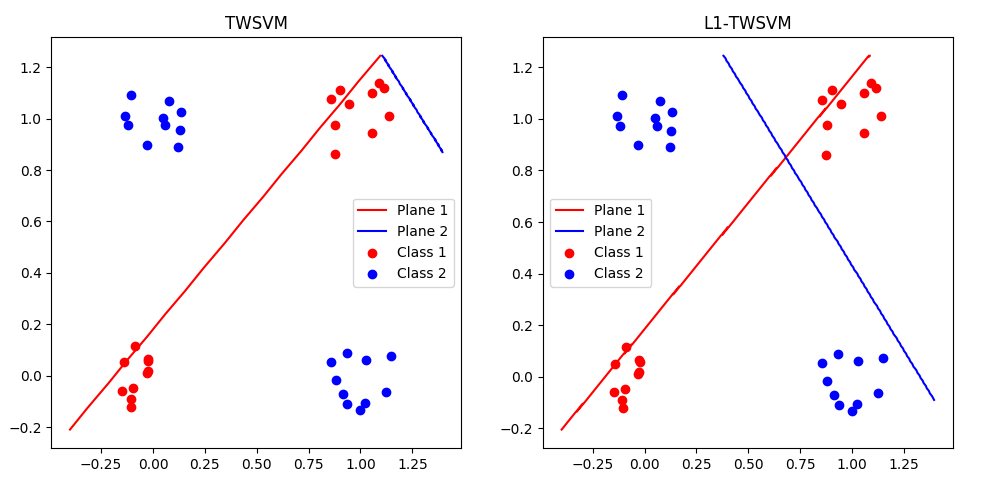
\includegraphics[width=0.8\textwidth]{./img/without_norm_cons.png}
\caption{不带离群点,无参数规范化}
\label{no_out_no_reg}
\end{figure}

\begin{figure}[ht]
\centering
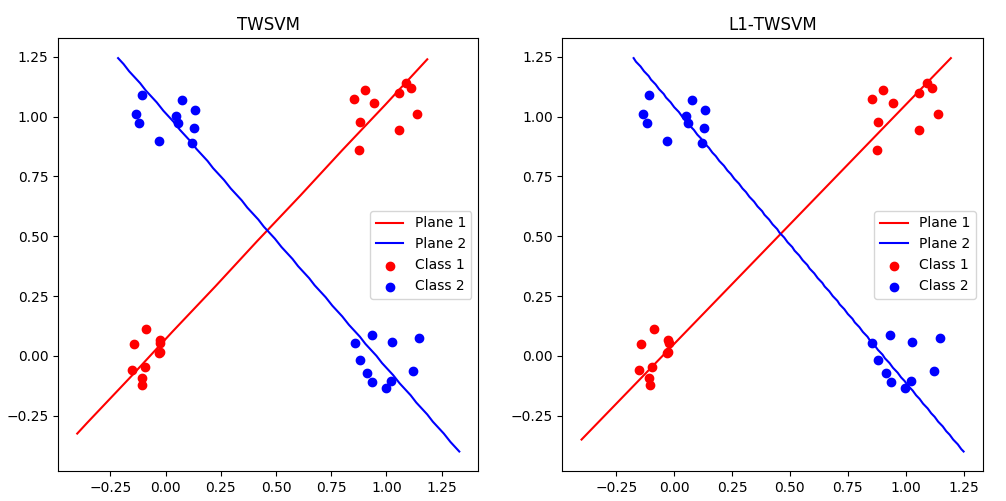
\includegraphics[width=0.8\textwidth]{./img/without_outliers.png}
\caption{不带离群点,参数规范化}
\label{no_out}
\end{figure}

增加离群点再进行实验,拟合结果如图 \ref{outliers}。可见离群点使 $l_2$-范数下的超平面产生较大的偏移,而 L1-TWSVM 拟合的直线受影响较小。实验结果说明,与 TWSVM 相比,L1-TWSVM 确实能够减小离群点对拟合超平面的影响。

\begin{figure}[ht]
\centering
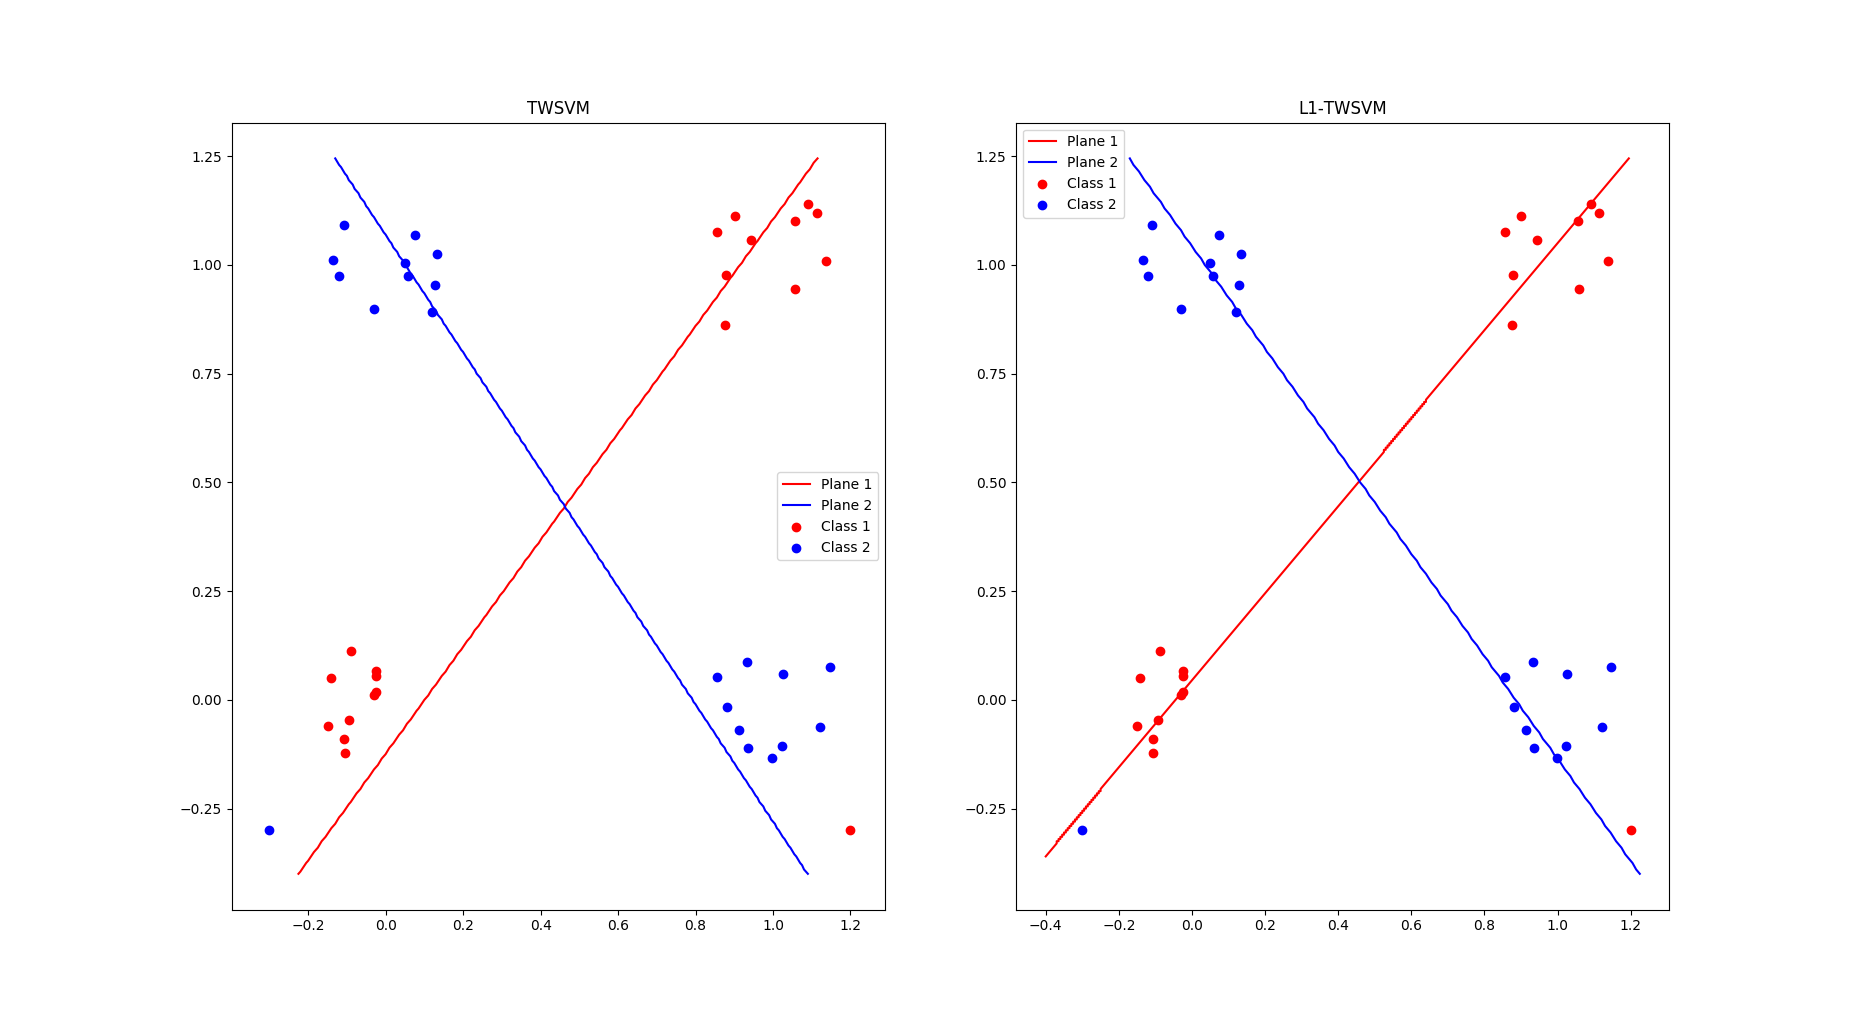
\includegraphics[width=0.8\textwidth]{./img/with_outliers.png}
\caption{带离群点,参数规范化}
\label{outliers}
\end{figure}

\section{总结}

本次作业本组阅读了 \parencite{yan2018efficient},对其中的算法提出思路,算法收敛性证明进行了整理。最后使用 \verb|Python| 进行了数值实验,验证了算法 L1-TWSVM 的正确性。


\printbibliography[heading=bibintoc, title=参考文献]

\appendix
\section{实验代码}
\label{append_code}
\verbatiminput{./codes/main.py}


\end{document}
